% Page du titre
%
\expandafter\newgeometry\expandafter{\thegeometryextra,headheight=0pt,marginparwidth=0pt,textwidth=7in,textheight=10in}
\begin{titlepage}\noindent{%
\thispagestyle{emptynonum}%
% logo
\begin{minipage}{0.2\textwidth}%
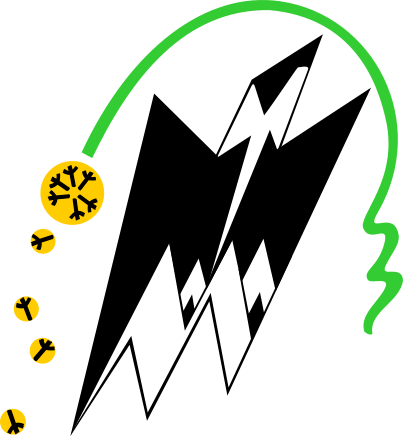
\includegraphics[width=1.1in]{univ-logo.png}
\end{minipage}% no new line
\begin{minipage}{0.8\textwidth}
\raggedleft
{
\bfseries
%\scriptsize
\footnotesize
\setstretch{1.0}
République Algérienne Démocratique et Populaire\\
Ministère de l'Enseignement Supérieur et de la Recherche Scientifique\\
Université Mouloud Mammeri de Tizi-Ouzou\\
Faculté de Génie Électrique et d'Informatique\\
Département d'Informatique\\
}
\end{minipage}%
% spacing
\par
\vspace*{1.0in}
%
\noindent{\begin{center}%
	\noindent{\shadowoffset{2pt}\shadowtext{\bfseries\Huge THÈSE}}\\
	\vspace*{10pt}
	\noindent{\large En vue de l'obtention du diplôme \\
	de Master 2 en Informatique}\\
	\vspace*{5pt}
	\noindent{\large\textnormal{Spécialité:} Systèmes Informatiques}\\
	\vspace*{25pt}
	\noindent{\large\textnormal{Présenté par:} {\bfseries\Large \theauthor}}\\
	\vspace*{5pt}
\end{center}}
% title
\noindent{\centering \begin{tcolorbox}[width=6in,
			text width=5.8in,
			halign=center,
			arc=3pt,
			outer arc=4pt
			boxrule=2pt,
			colback=black!3!white
		  ]%%
                  \bfseries\LARGE \thetitlefrench
\end{tcolorbox}}%
%
\vspace*{0pt}%
\noindent{\begin{center}\begin{minipage}{6.0in}\raggedleft\large{}\textnormal{Mémoire encadré par:} \theadvisor\end{minipage}\end{center}}
\par
%
\vspace*{30pt}
\noindent{\begin{center}\begin{minipage}{6.0in}\large{}Soutenu publiquement devant le jury composé de:\end{minipage}\end{center}}
\par
%
\begin{center}
	\setstretch{1.4}
	\large 
	\begin{tabularx}{6in}{l>{\arraybackslash\hspace{0.5in}}Xr}%{l>{\centering\arraybackslash}Xr}
		\hline
		Prénom NOM			& Pr. Univ. de Tizi-Ouzou	&	Président\\
		Prénom NOM			& MAA. Univ. de Tizi-Ouzou	&	Examinateur\\
		Prénom NOM			& MCA. Univ. de Tizi-Ouzou 	&	Examinateur\\
		\theadvisor			& MCB. Univ. de Tizi-Ouzou	&	Encadrant\\
		\hline
	\end{tabularx}
\end{center}
